\documentclass[12pt]{article}
\usepackage[top=1in, bottom=1in, right=1in, left=1in]{geometry}
\usepackage{setspace}
\usepackage{graphicx}
\usepackage{setspace}
\usepackage{parskip}
\usepackage{url}

\title{Theory of Schedule C Appointments}
\date{May 7, 2015}
\author{Emily H. Moore}

\usepackage{Sweave}
\begin{document}
\Sconcordance{concordance:MooreScheduleCTheoryPaper.tex:MooreScheduleCTheoryPaper.Rnw:%
1 12 1 1 0 61 1}

\maketitle
\parindent=0.5in
\parskip=0.01in
\doublespacing

President Taft once said ``every time I make an appointment I create nine enemies and one ingrate'' (Pfiffner 2015). It takes millions of employees to run the federal bureaucracy and the difficult and often controversy-inspiring task of appointing several thousand of them rests with the president. The most visible of these are presidentially-appointed, Senate-confirmed positions. As Lewis and Waterman (2013) note, almost all studies focus on these high-profile personnel. Certainly, journalists have mainly studied appointees via the advice and consent process, but even scholars, who have broadened their scope beyond only traditional top level appointees have largely ignored lower level employees. Doing so misses an important part of administrative politics. 

Clearly Senate-confirmed appointees are important policymakers, but the president's administration has a definite need for other types of employees as well, especially considering the increasing length of time to confirmation and the consequently shrinking amount of time these appointees serve. As Pfiffner points out, it took fewer than 2.5 months for John F. Kennedy's appointees to make it through the advice and consent process, but George Bush's appointees waited nearly nine months to begin serving. While Ronald Reagan managed to appoint 86 percent of the top appointees in his first year, Obama could not complete two-thirds. Partially as a result of this, the average time in office for these political appointees is only 2.5 years. It would seem ideal for all employees in the government, and particularly those with policy-making authority, to undergo a vetting process such as advice and consent, but the sheer volume of appointees and polarization in Congress quickly dissolves this notion. Clearly, the administration requires a way to staff the bureaucracy quickly and with a certain amount of flexibility.

Thus, one of the administration's key advantages is its ability to hire low-level bureaucrats. These employees have considerable influence over policy and largely slip under the radar of congressional and media oversight (Lewis and Waterman 2013). This is partly because the president's advisors choose who to appoint to these positions without congressional approval. Still, these appointments are perfectly legal exercises of the administration's power with which Congress is complicit, and while low-level appointees certainly serve in political capacities, they also perform other functions. For example, appointees play an essential informational role which benefits both Congress and the president (Gailmard and Patty 2012). Additionally, appointees serve in a simple functional capacity, existing, in part, to help execute policy day-to-day. Given finite resources to complete policy tasks (and particularly finite because only some appointments are flexible), which agencies receive these valuable low-level appointees? How are they used?

Previous scholars have focused on how appointment power confers political control, but low-level employment patterns also provide information about the administrations's \textit{attentiveness} to a particular agency---an angle left unstudied in previous research. Yet policy attention, especially as conducted through more flexible manpower, is one of the most limited resources. Students of bureaucracy should take note of how administrations allocate their policy attention through lower-level bureaucrats. In this paper, I describe the nature of Schedule C appointees and develop a simple theory for understanding the Schedule C process in order to aid further investigations.

\section{Schedule C Appointments}


When most people think of presidential appointments, they think of the advice and consent process. Of course, employees hired in this way (known as PAS appointments to the Office of Personnel Management) make up a meager portion of federal employment. In fact, as of June 2014, there were over two million appointees to federal agencies and only about 1,200 PAS appointments. Beyond traditional PAS and the competitive service, there is still another class of appointments: excepted service. Excepted service positions are technically those appointments that have been excepted from competition via the competitive service. These positions are also excepted from advice and consent, so the president and his office hires these employees without Senate approval.

Some excepted service appointments are reserved for positions for which the Office of Personnel Management (OPM) does not or cannot provide a test or standard (professionals such as lawyers are one example). Other excepted service appointments are reserved for those with disabilities or are set aside for interns. These appointments, like competitive service appointments, are largely used to complete the day-to-day operations of the government. However, there is one particular class of excepted service appointments which is explicitly political. OPM describes Schedule C appointments as those positions of a ``confidential'' or ``policy-determining nature,'' for which it is important the employee shares the president's vision for the agency. 

To provide some context, President Eisenhower created Schedule C appointments when he first reached office. According to Gailmard and Patty (2012), Eisenhower instituted Schedule C because he was faced with the political realities of being the first Republican to win the presidency in twenty years (leaving him with few trusted advisors) and because the post-World War II era left him with an expansive administrative state, which reached further into the economy and society than had previously been conceived. Schedule C was designed to exist between other classes of appointments---appointees beholden to the administration, but who did not undergo advice and consent or competitive service processes.  

As an example of these appointments today, the Administrator and Deputy Administrator of the EPA are both Senate-confirmed appointees. The EPA's Special Assistant to the Senior Climate Policy Counsel is a Schedule C position as is the White House Liaison. Similarly, the Chairmen of the Council on Environmental Quality is a PAS appointment, while the Special Assistant on Climate Change is a Schedule C appointment. Thus, while the highest positions are Senate-confirmed, they are quickly followed by lower-level, but still important Schedule C appointments. 

Schedule C appointments can be mandated by law, but what makes them so special is that they are almost entirely positions which the administration creates.\footnote{Occasionally, when  Congress creates an agency, it will specify that a position be excepted service or will allow for a certain number of excepted positions. Usually, though, the administration initiates the creation of a position.} When the a supervisor within an agency wishes to hire someone via Schedule C, he files papers with OPM indicating the individual appointment and the scope of the position. When this person is fired or quits, the position is dissolved. If the supervisor wishes to hire another person to fulfill the role, he must ``create" the position anew. In other words, Schedule C appointees are not filling a statutory position; they are filling the administration's current needs. This makes Schedule C appointments particularly suited to considering policy attention.

Very little research discusses, much less focuses on, Schedule C appointments. This is surprising considering that, while these individuals make up a small proportion of federal employment, they make up a considerable portion of presidential appointees. In fact, Schedule C employees typically make up at least 15 percent of the appointments the president must make in the Plum Book. In one of the few treatments of Schedule C, Lewis and Waterman (2013) refer to them as ``the invisible appointments" largely because of their lack of media and scholarly attention. As such, greater systematic treatment is needed to better understand their purpose for the president and their impact on policy. 

\section{Developing a Theory}

As mentioned before, there is no theory as yet for explaining Schedule C appointees and their role within the government apparatus. As such, it is important to develop a framework for understanding how Schedule C appointees fit into the bureaucractic policymaking process.

\begin{figure}
\centering
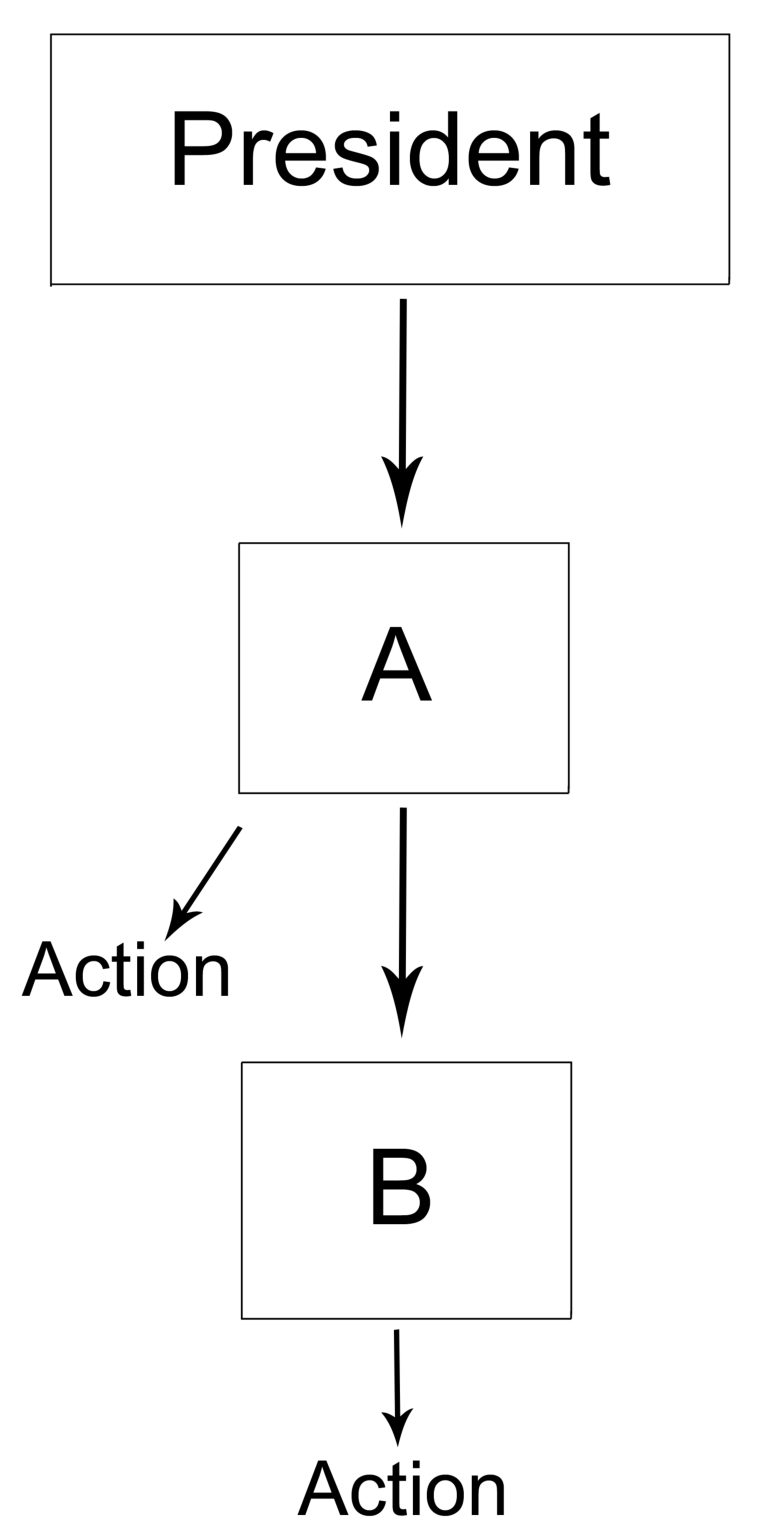
\includegraphics[height=5in,width=3in]{ModelV1.pdf}
\end{figure}

Figure 1 shows a simple diagram of a lower-level appointee process. First, the president chooses A. Appointee A can be thought of as a PAS appointee such as the Secretary of State or the top Administrator of the EPA. Next, Appointee A has a decision. He or she may choose to appoint an underling, B, or not. To some extent, Appointee A's actions represent the productivity of the agency which he or she heads. As such, A may choose to take some action (for example, make a new rule). Appointee B may also take some action that can benefit both Appointee A and the agency itself and also, indirectly, the President. We might be interested in the extent to which B actually performs some actions---if she does not, then perhaps she is merely a patronage appointment. On the other hand, if B is very active and especially if B's actions are coordinated with A's, we know that A and B are coordinating to advance policy within the agency. In particular, their coordinated actions are not merely delegation. 

One might conceivably extend this model further as is visible in Figure 2. Suppose, for example, that we consider multiple agency heads (represented by A1 and A2). These agency heads may differ in the amount of support (the numbers of Bs) that they attract or require. Moreover, the contributions of the B appointees may differ.

\begin{figure}
\centering
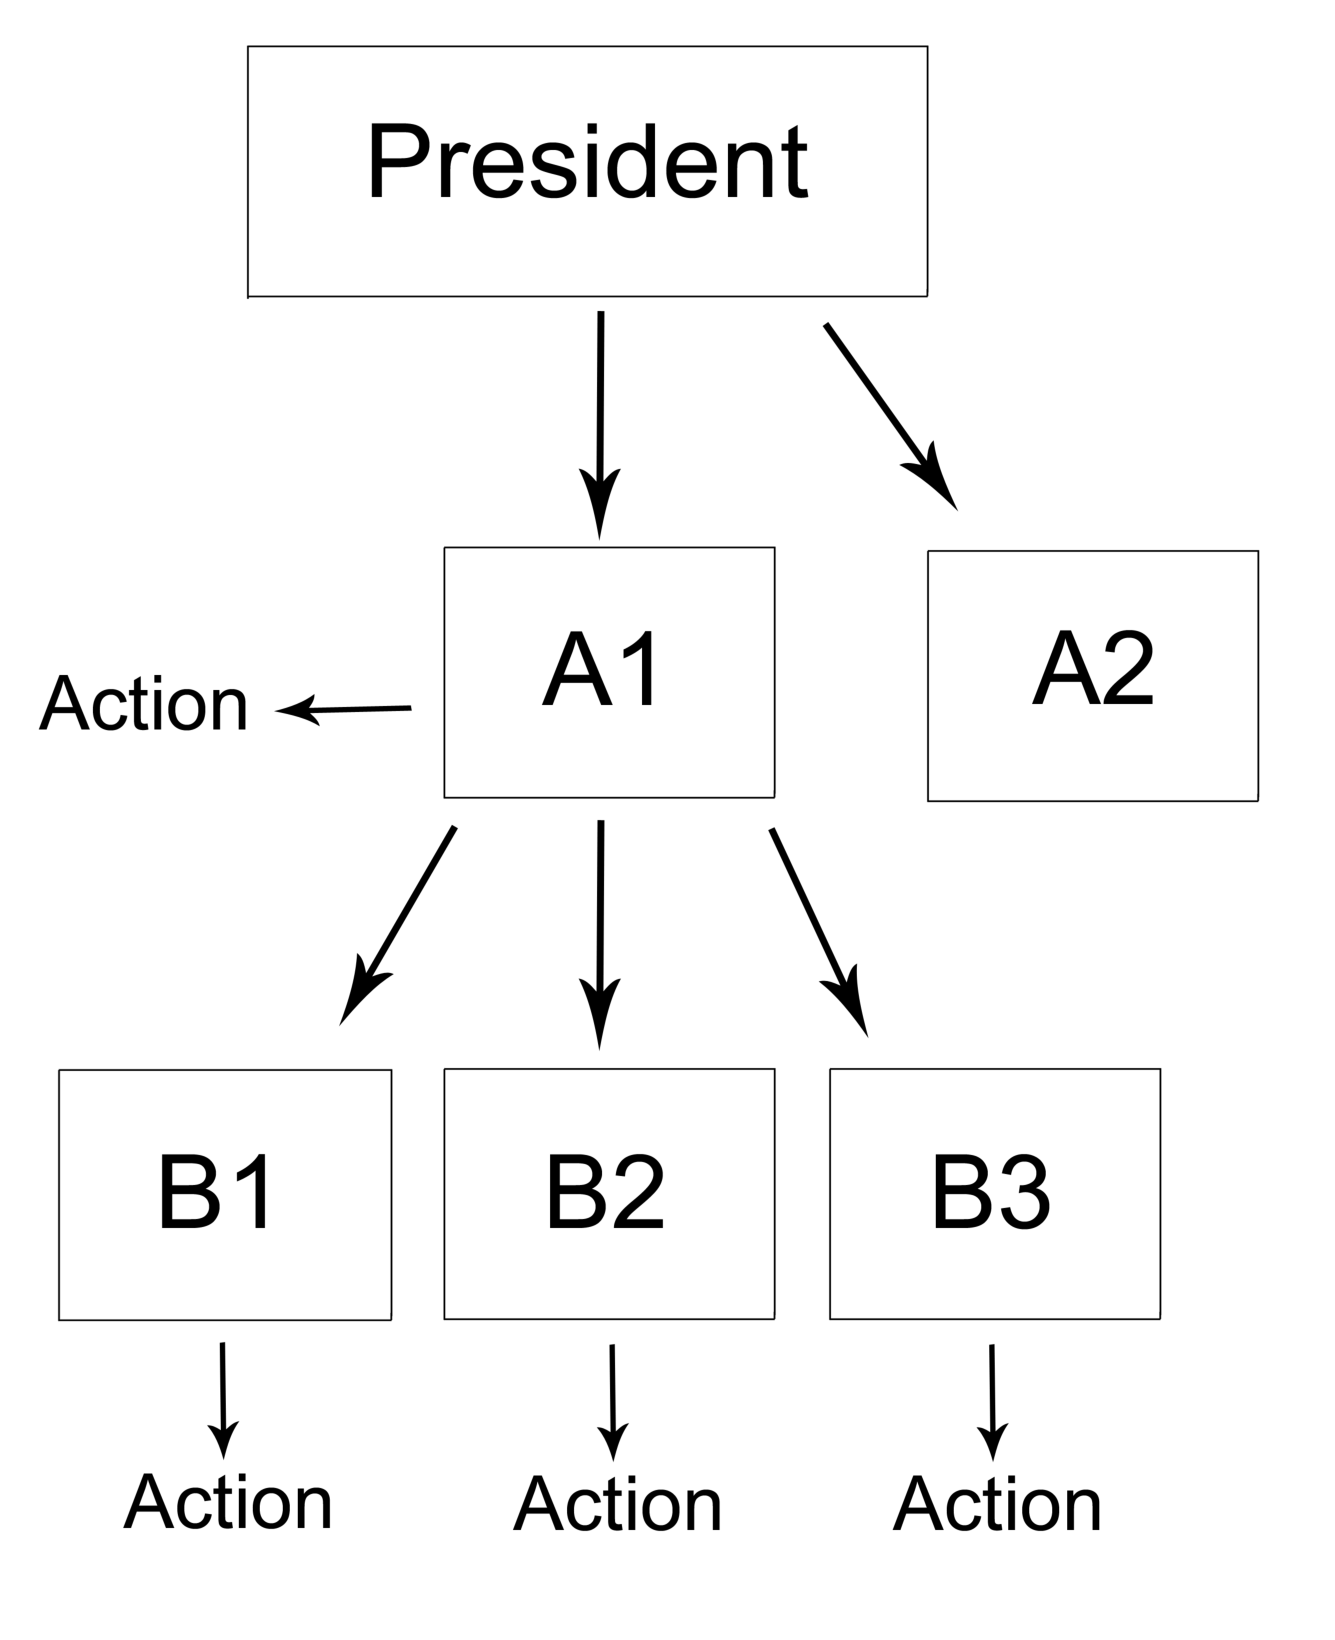
\includegraphics[height=5in,width=4.5in]{ModelV3.pdf}
\end{figure}

Insofar as Appointee B's actions are coordinated with those of Appointee A, we can get a sense of policy attention. In other words, so long as the B appointees are doing something, we can get a sense of the administration's attention to a particular policy area--not just in terms of the rules it produces (via the A appointees), but also in terms of the number of Schedule C appointees who work within. Because the A appointees \textit{choose} whether or not to hire B appointees and have broad authority over who gets hired and when, this is arguably much more important than the overall size of the rest of the staff or even other political appointees who are required to serve by law.

Thankfully, the Federal Register offers a reasonable way to test this framework. Because all new Schedule C authorities (and revoked authorities) are published there, we can get a good sense of the extent to which the ``A"s appoint the ``B"s. We can also get a good sense of the number of rules and notices that come out of agencies--A's actions. As such, we may be able to study topics of considerabl interest--such as whether or not agencies with more Schedule C appointments are more productive than those without. 

\section{References}
\noindent \hangindent=0.7cm Gailmard, Sean and John W. Patty. 2012. \textit{Learning While Governing.} Chicago: University of Chicago Press. 

\noindent \hangindent=0.7cm Lewis, David, E and Richard W. Waterman. 2013. ``The Inivisible Presidential Appointments: An Examination of Appointments to the Department of Labor, 2001-11.'' \textit{Presidential Studies Quarterly} 43(1): 35-57.

\noindent \hangindent=0.7cm Pfiffner, James P. 2015. ``Presidential Appointments and Managing the Executive Branch." Political Appointee Project. \url{http://www.politicalappointeeproject.org/commentary/appointments-and-managing-executive-branch} (April 9, 2015).



\end{document}
